\documentclass[12pt]{article}\usepackage[]{graphicx}\usepackage[]{xcolor}
% maxwidth is the original width if it is less than linewidth
% otherwise use linewidth (to make sure the graphics do not exceed the margin)
\makeatletter
\def\maxwidth{ %
  \ifdim\Gin@nat@width>\linewidth
    \linewidth
  \else
    \Gin@nat@width
  \fi
}
\makeatother

\definecolor{fgcolor}{rgb}{0.345, 0.345, 0.345}
\newcommand{\hlnum}[1]{\textcolor[rgb]{0.686,0.059,0.569}{#1}}%
\newcommand{\hlsng}[1]{\textcolor[rgb]{0.192,0.494,0.8}{#1}}%
\newcommand{\hlcom}[1]{\textcolor[rgb]{0.678,0.584,0.686}{\textit{#1}}}%
\newcommand{\hlopt}[1]{\textcolor[rgb]{0,0,0}{#1}}%
\newcommand{\hldef}[1]{\textcolor[rgb]{0.345,0.345,0.345}{#1}}%
\newcommand{\hlkwa}[1]{\textcolor[rgb]{0.161,0.373,0.58}{\textbf{#1}}}%
\newcommand{\hlkwb}[1]{\textcolor[rgb]{0.69,0.353,0.396}{#1}}%
\newcommand{\hlkwc}[1]{\textcolor[rgb]{0.333,0.667,0.333}{#1}}%
\newcommand{\hlkwd}[1]{\textcolor[rgb]{0.737,0.353,0.396}{\textbf{#1}}}%
\let\hlipl\hlkwb

\usepackage{framed}
\makeatletter
\newenvironment{kframe}{%
 \def\at@end@of@kframe{}%
 \ifinner\ifhmode%
  \def\at@end@of@kframe{\end{minipage}}%
  \begin{minipage}{\columnwidth}%
 \fi\fi%
 \def\FrameCommand##1{\hskip\@totalleftmargin \hskip-\fboxsep
 \colorbox{shadecolor}{##1}\hskip-\fboxsep
     % There is no \\@totalrightmargin, so:
     \hskip-\linewidth \hskip-\@totalleftmargin \hskip\columnwidth}%
 \MakeFramed {\advance\hsize-\width
   \@totalleftmargin\z@ \linewidth\hsize
   \@setminipage}}%
 {\par\unskip\endMakeFramed%
 \at@end@of@kframe}
\makeatother

\definecolor{shadecolor}{rgb}{.97, .97, .97}
\definecolor{messagecolor}{rgb}{0, 0, 0}
\definecolor{warningcolor}{rgb}{1, 0, 1}
\definecolor{errorcolor}{rgb}{1, 0, 0}
\newenvironment{knitrout}{}{} % an empty environment to be redefined in TeX

\usepackage{alltt}


\usepackage[hmargin=1in,vmargin=1in]{geometry}
\usepackage{parskip}
\usepackage{hyperref}
\usepackage{graphicx}
\hypersetup{pdfstartview=FitV,hidelinks}




\IfFileExists{upquote.sty}{\usepackage{upquote}}{}
\begin{document}

{
  \Large
  \centering
  Lab 4 Assignment --- Stochasticity and Extinction \par
  % \large
  \normalsize
  % Submit your Excel file and R script before Monday.
  % \normalsize
  Answer each of the following questions and upload your completed Excel
  file and R script to ELC by 8:00am on Monday. Be sure to show your
  calculations. Undergrads only need to do the \textit{second}
  exercise in R, not the first. \\
}

\vspace{12pt}

{\bf Random Numbers in Excel \\}

\begin{figure}[h]
  \centering
  \fbox{
    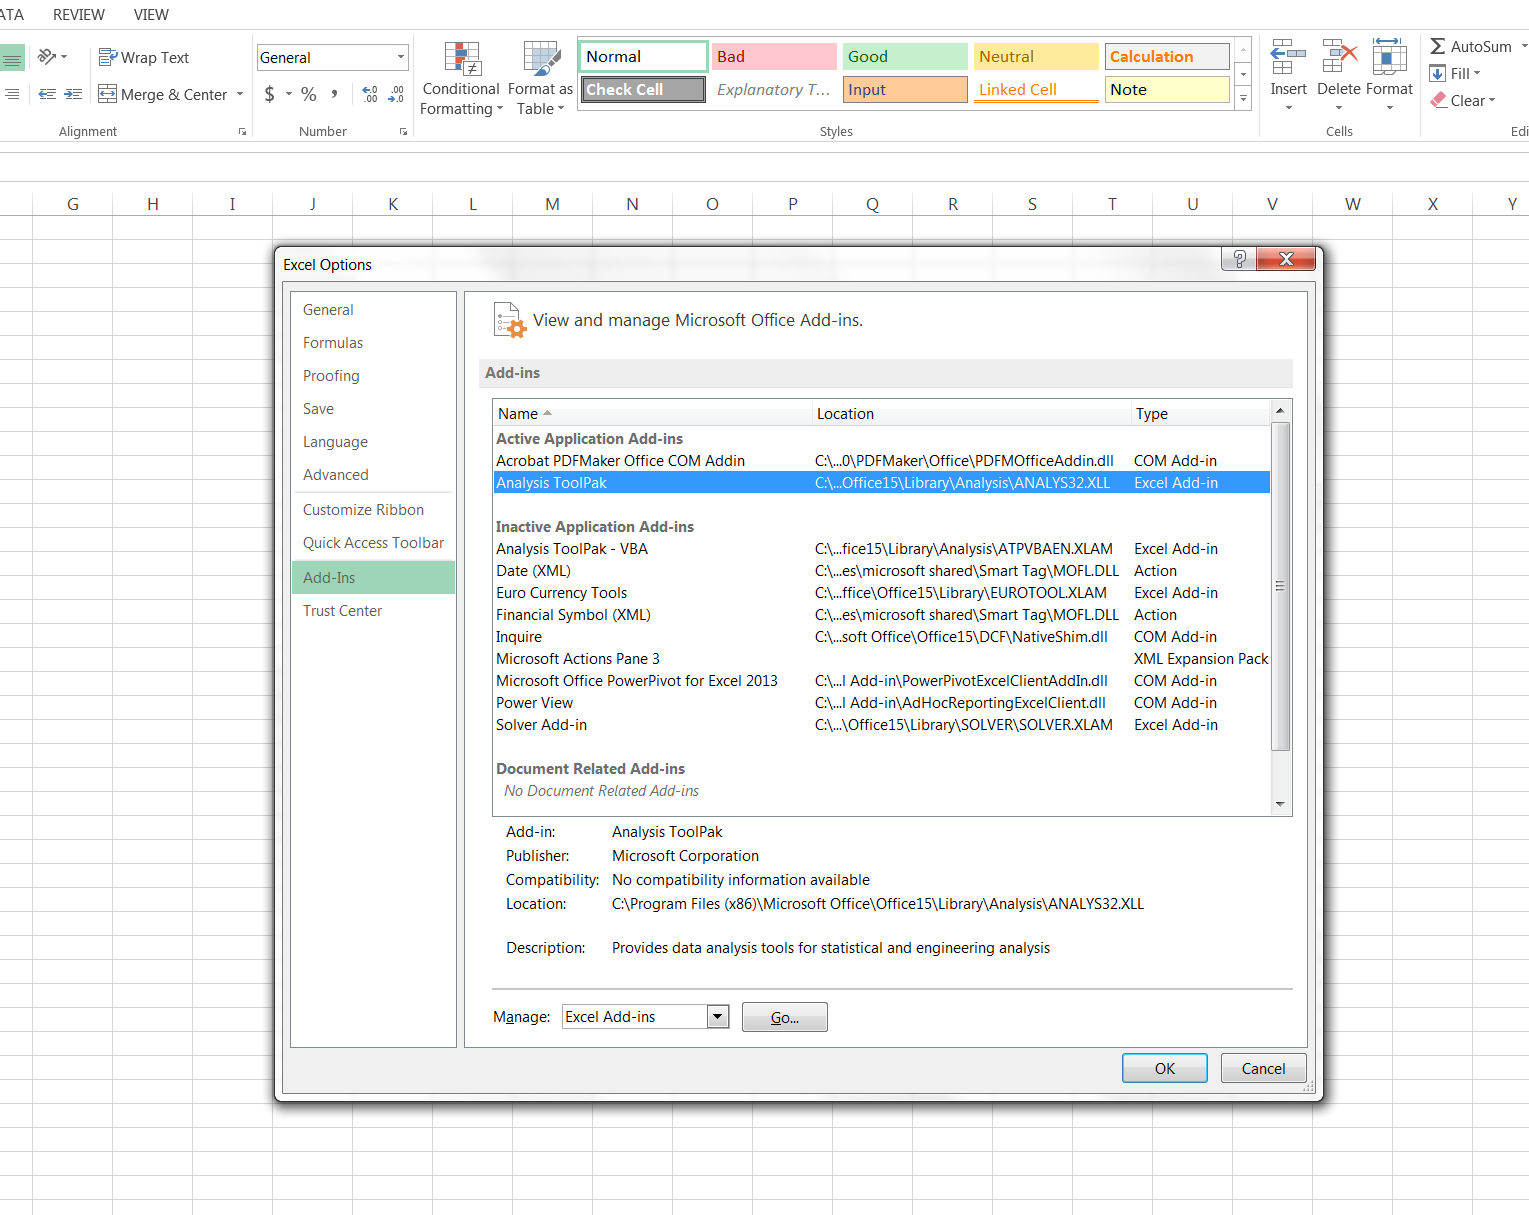
\includegraphics[width=0.95\textwidth]{figs/Excel-RNG}
  } \\
  \caption{To generate random numbers in Excel, you must load the
    ``Analysis Toolpak'' add-in by clicking
    {\tt File $>$ Options $>$ Add-Ins $>$ Analysis Toolpak}. Then hit
    ``Go'' (not ``OK'') and select ``Analysis Tookpak'' again.}
  \label{fig:rng}
\end{figure}

\clearpage

\begin{figure}[h]
  \centering
  \fbox{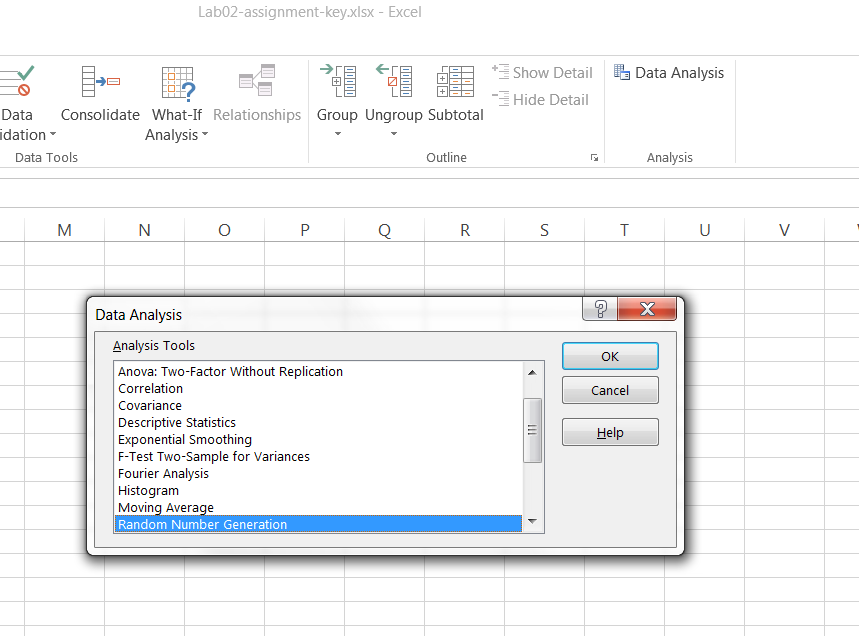
\includegraphics[width=0.6\textwidth]{figs/Excel-RNG-2}}
  \caption{\footnotesize Once the Analysis ToolPak is installed, you can generate
    random numbers by clicking the ``Data Analysis'' button in the
    ``Data'' tab.
  }
  \label{fig:rng-2}
\end{figure}

\vspace{1cm}

\begin{figure}[h]
  \centering
  \fbox{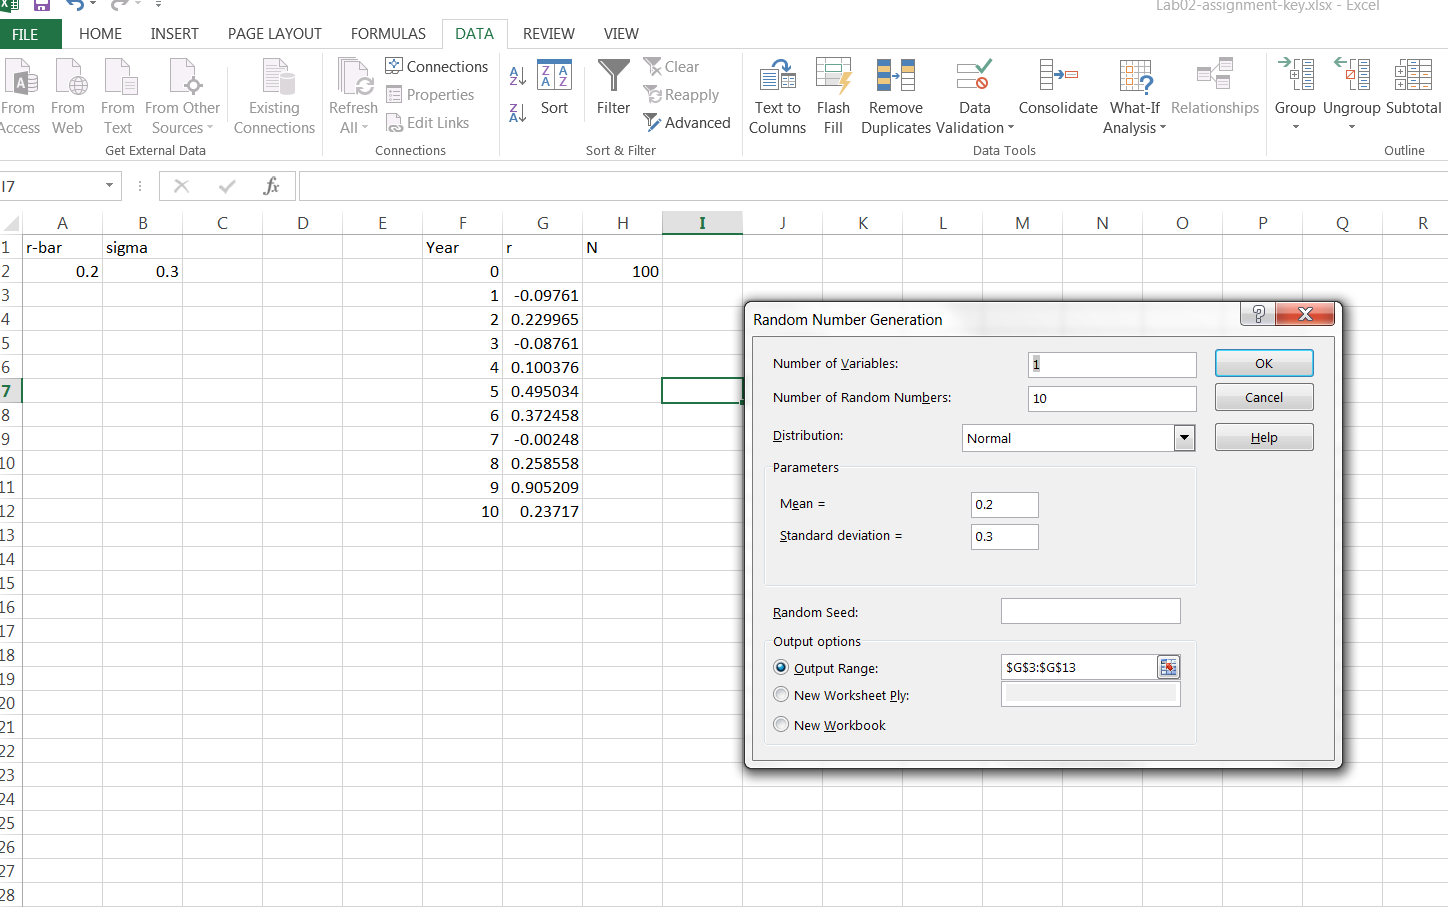
\includegraphics[width=0.6\textwidth]{figs/Excel-RNG-3}}
  \caption{\footnotesize We will use three distributions: Normal,
    Binomial, and Poisson. The latter two are only used in Exercise
    II. Note: You can think of the ``number of variables'' as the
    number of columns of random variables, and the ``number of random
    numbers'' as the number of cells in each column.
  }
  \label{fig:rng-3}
\end{figure}


\clearpage


% \vspace{12pt}

{\bf Exercise I \\}
\begin{enumerate}
  \item[(A)] Suppose a population is growing geometrically with
    $r=-0.2$ and $N_0=500$. There is no random variation, and
    quasi-extinction occurs when $N$ falls below 20 individuals.
    What is the time to quasi-extinction ($T_e$)? In other words, how
    long will it take for the population to fall below 20 individuals?
  % \item Now imagine that there is no demographic stochasticity,
  %   but environmental stochasticity occurs with $X_t \sim
  %   \mathrm{Normal}(\mu=0, \sigma=10)$, where $\mu$ is the mean
  %   and $\sigma$ is the standard deviation of the random variable
  %   $X$. Generate the random values of $X$ that will be
  %   used in the 10 simulations in the next step.
  \item[(B)] Now imagine that there is no demographic stochasticity,
    but environmental stochasticity occurs with $r_t \sim
    \mathrm{Normal}(\mathrm{mean}=-0.2, \mathrm{SD}=0.05)$. Generate
    the random values of $r_t$ that will be  
    used in the 10 simulations in the next step.
  \item[(C)] Conduct 10 simulations over a 30 year time period, and force
    the population size to zero after it falls below the threshold.
    This can be done by multiplying the geometric
    growth equation by a ``test statement'', like this:
    {\tt =(EQUATION)*(CELL>20)}, where {\tt EQUATION} should be
    replaced with the population growth equation and {\tt CELL} should
    be replaced with the cell reference for abundance at the previous
    time step. Plot the projections.
  \item[(D)] What is the average $T_e$ based on these 10 simulations?
  \item[(E)] What is extinction risk at year 15?
\end{enumerate}

% \vspace{12pt}


% {\bf Exercise II \\}
% \begin{enumerate}
%   \item Simulate 10 populations under a logistic growth model with
%     $N_0$=20, $K$=40, and a normally-distributed growth rate $r_{\mathrm{max}_t}
%     \sim \mathrm{Norm}(\mu=0.1, \sigma=0.2)$. Assume that the
%     quasi-extinction threshold is equal to 10, and force the
%     population size to zero if it falls below the threshold using a
%     test statement as before. Plot the projections.
%   \item What are the quasi-extinction risks at years 5, 10, and 15?
% \end{enumerate}


\newpage


{\bf Exercise II \\ }
% In this exercise, you will be exposed to two new probability
% distributions: the Poisson and the binomial. The Poisson distribution
% is useful for data that are non-negative integers. It only has
% a single parameter (often called ``lambda'' but not to be confused with the
% finite rate of increase) that describes the expected value of the
% count data. In stochastic population models, the Poisson distribution
% can be used to model the number of births ($B_t$) that occur in a time
% interval. 

% The binomial distribution is also useful for data that are
% non-negative integers, but it has an upper bound. In population
% models, the upper bound is often population size, and we use the model
% to describe how many individuals die during some time period.

Assume that a population is geographically closed such that there is
no immigration or emigration. The number of individuals born is a
Poisson random variable:
\[
  B_t \sim \mathrm{Poisson}(N_t \times b)
\]
and the number that die each year is a binomial random variable:
\[
  D_t \sim \mathrm{Binomial}(N_t, d)
\]
Abundance is just the number that were alive plus the number that were
born, minus the number that died:
\[
  N_{t+1} = N_t + B_t - D_t
\]
\begin{enumerate}
  \item[(A)] Beginning with $N_0=300$, conduct one simulation over 5
    years, in which $b=0.3$ and $d=0.2$. Plot the simulated values of
    abundance over time. Hint: You have  to randomly generate $B_t$
    and $D_t$ before you can compute  $N_{t+1}$, one year at a time.
  \item[(B)] Do you think this population will reach a stochastic
    equilibrium? Why or why not? (A stochastic equilibrium occurs when
    a population fluctuates around a long-term average).
  \item[(C)] Can population size ever be less than zero under this model?
    Why or why not?
  \item[(D)] Do another simulation, but this time make the mortality rate
    ($d$) density-dependent according to the model $d_t = 0.2 +
    0.001\times N_t$. Will this population reach a stochastic equilibrium? If
    so, at what value of abundance does the equilibrium point occur?
\end{enumerate}


\newpage

{\bf Example {\tt R} code \\}

% Geometric growth with environmental stochasticity
% <<geom-stoch,out.width="0.75\\textwidth",fig.align='center',size='normalsize',echo=-1>>=
% set.seed(430)
% r <- -0.1
% sigma <- 5
% nYears <- 50
% extinctionThreshold <- 10

% ## Repeat the next steps 10 times to do 10 simulations
% ## Or, do a 'nested for loop' and save each simulation (harder)
% N1 <- rep(NA, nYears)  ## Population size 
% X <- rep(NA, nYears)   ## Random variable for environmental stochasticity
% N1[1] <- 100           ## Initial population size
% for(t in 2:nYears) {
%     X[t-1] <- rnorm(n=1, mean=0, sd=sigma)
%     N1[t] <- (N1[t-1] + N1[t-1]*r + X[t-1])*(N1[t-1]>extinctionThreshold)
% }
% plot(1:nYears, N1, xlab="Time", ylab="Abundance", type="b")
% @ 


Geometric growth with environmental stochasticity
\begin{knitrout}
\definecolor{shadecolor}{rgb}{0.969, 0.969, 0.969}\color{fgcolor}\begin{kframe}
\begin{alltt}
\hldef{rbar} \hlkwb{<-} \hlnum{0}
\hldef{sigma} \hlkwb{<-} \hlnum{0.5}
\hldef{nYears} \hlkwb{<-} \hlnum{50}
\hldef{extinctionThreshold} \hlkwb{<-} \hlnum{10}

\hlcom{## Repeat the next steps 10 times to do 10 simulations}
\hlcom{## Or, do a 'nested for loop' and save each simulation (harder)}
\hldef{N1} \hlkwb{<-} \hlkwd{rep}\hldef{(}\hlnum{NA}\hldef{, nYears)}  \hlcom{## Population size }
\hldef{N1[}\hlnum{1}\hldef{]} \hlkwb{<-} \hlnum{50}            \hlcom{## Initial population size}
\hldef{r} \hlkwb{<-} \hlkwd{rep}\hldef{(}\hlnum{NA}\hldef{, nYears}\hlopt{-}\hlnum{1}\hldef{)}
\hlkwa{for}\hldef{(t} \hlkwa{in} \hlnum{2}\hlopt{:}\hldef{nYears) \{}
    \hldef{r[t}\hlopt{-}\hlnum{1}\hldef{]} \hlkwb{<-} \hlkwd{rnorm}\hldef{(}\hlkwc{n}\hldef{=}\hlnum{1}\hldef{,} \hlkwc{mean}\hldef{=rbar,} \hlkwc{sd}\hldef{=sigma)}
    \hldef{N1[t]} \hlkwb{<-} \hldef{(N1[t}\hlopt{-}\hlnum{1}\hldef{]} \hlopt{+} \hldef{N1[t}\hlopt{-}\hlnum{1}\hldef{]}\hlopt{*}\hldef{r[t}\hlopt{-}\hlnum{1}\hldef{])}\hlopt{*}\hldef{(N1[t}\hlopt{-}\hlnum{1}\hldef{]}\hlopt{>}\hldef{extinctionThreshold)}
\hldef{\}}
\hlkwd{plot}\hldef{(}\hlnum{1}\hlopt{:}\hldef{nYears, N1,} \hlkwc{xlab}\hldef{=}\hlsng{"Time"}\hldef{,} \hlkwc{ylab}\hldef{=}\hlsng{"Abundance"}\hldef{,} \hlkwc{type}\hldef{=}\hlsng{"b"}\hldef{)}
\end{alltt}
\end{kframe}

{\centering \includegraphics[width=0.75\textwidth]{figure/geom-stoch-1} 

}


\end{knitrout}


\newpage

Poisson-Binomial birth-death model

\begin{knitrout}
\definecolor{shadecolor}{rgb}{0.969, 0.969, 0.969}\color{fgcolor}\begin{kframe}
\begin{alltt}
\hldef{b} \hlkwb{<-} \hlnum{0.15}  \hlcom{## Birth rate}
\hldef{d} \hlkwb{<-} \hlnum{0.2}   \hlcom{## Mortality rate}
\hldef{nYears} \hlkwb{<-} \hlnum{50}
\hldef{N2} \hlkwb{<-} \hlkwd{rep}\hldef{(}\hlnum{NA}\hldef{, nYears)}  \hlcom{## Empty vector for population size }
\hldef{B} \hlkwb{<-} \hlkwd{rep}\hldef{(}\hlnum{NA}\hldef{, nYears)}   \hlcom{## Random variable for nBirths}
\hldef{D} \hlkwb{<-} \hlkwd{rep}\hldef{(}\hlnum{NA}\hldef{, nYears)}   \hlcom{## Random variable for nDeaths}
\hldef{N2[}\hlnum{1}\hldef{]} \hlkwb{<-} \hlnum{100}           \hlcom{## Initial population size}
\hlkwa{for}\hldef{(t} \hlkwa{in} \hlnum{2}\hlopt{:}\hldef{nYears) \{}
    \hldef{B[t}\hlopt{-}\hlnum{1}\hldef{]} \hlkwb{<-} \hlkwd{rpois}\hldef{(}\hlkwc{n}\hldef{=}\hlnum{1}\hldef{,} \hlkwc{lambda}\hldef{=N2[t}\hlopt{-}\hlnum{1}\hldef{]}\hlopt{*}\hldef{b)}
    \hldef{D[t}\hlopt{-}\hlnum{1}\hldef{]} \hlkwb{<-} \hlkwd{rbinom}\hldef{(}\hlkwc{n}\hldef{=}\hlnum{1}\hldef{,} \hlkwc{size}\hldef{=N2[t}\hlopt{-}\hlnum{1}\hldef{],} \hlkwc{prob}\hldef{=d)}
    \hldef{N2[t]} \hlkwb{<-} \hldef{N2[t}\hlopt{-}\hlnum{1}\hldef{]} \hlopt{+} \hldef{B[t}\hlopt{-}\hlnum{1}\hldef{]} \hlopt{-} \hldef{D[t}\hlopt{-}\hlnum{1}\hldef{]}
\hldef{\}}
\hlkwd{plot}\hldef{(}\hlnum{1}\hlopt{:}\hldef{nYears, N2,} \hlkwc{xlab}\hldef{=}\hlsng{"Time"}\hldef{,} \hlkwc{ylab}\hldef{=}\hlsng{"Abundance"}\hldef{,} \hlkwc{type}\hldef{=}\hlsng{"b"}\hldef{)}
\end{alltt}
\end{kframe}

{\centering \includegraphics[width=0.9\textwidth]{figure/pois-bin-1} 

}


\end{knitrout}


\end{document}

